\section{6 Degree of Freedom Manipulator}

\indent

To extrude a consistent bead of material along a surface, the extruder nozzle should be normal to the surface. This means that in flat layer printing, the extruder may always be held vertically above the print surface. However, curved layers may require the extruder to tilt and rotate to reach some areas properly. Thus, curved layer FDM 3D printing requires the extruder positioning mechanism to have more degrees of freedom than flat-layer printing. \\

The FANUC LR Mate 200iC 6 degree of freedom industrial robot arm provides the necessary degrees of freedom for curved layer printing. The robot was acquired as part of an eductional package that includes the robot, its housing, the controller, a gripper and vision system, and related softwrae. The robot is compact and has positioning repeatable to 0.02 mm. As such, the robot is a suitable platform for a curved layer 3D printer. The extruder will be mounted to the existing gripper, and the control electronics and filament will be mounted to the side of the robot cage. Figure~\ref{fig:robot} provides a photograph of the FANUC robot itself, while Figure~\ref{fig:robot with things} shows a photograph of the FANUC with the electronics board and extruder.\\

%% talk about speed / position tracking and built in language?

\begin{figure}[htp]
\centering
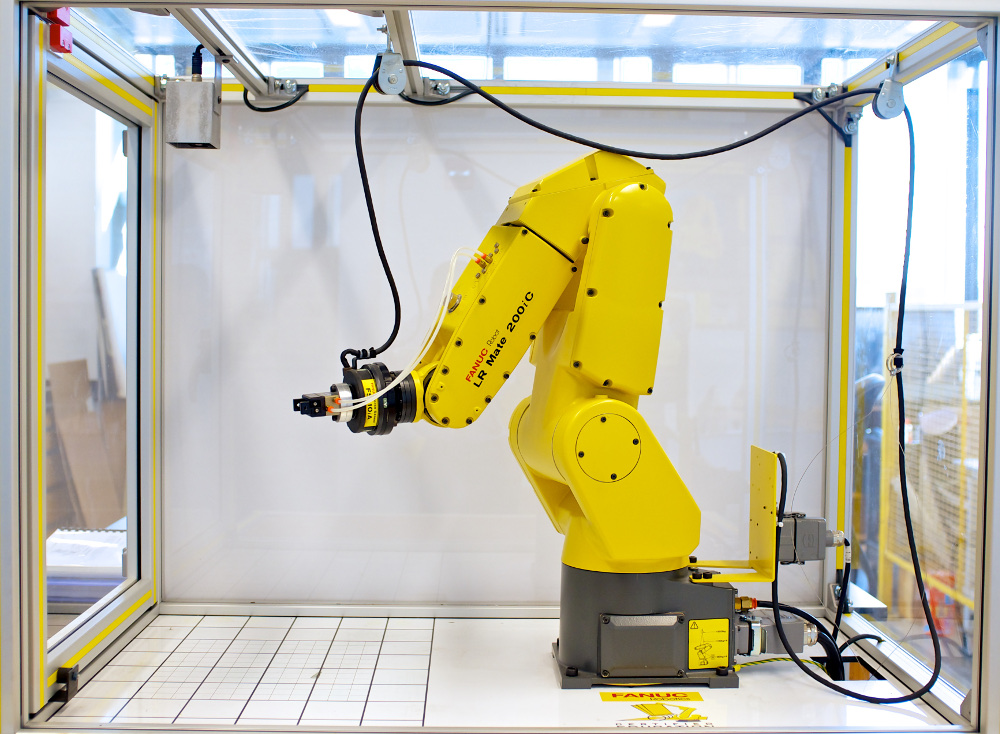
\includegraphics[width=0.5\textwidth]{./figures/robot}
\caption{A photograph of the FANUC LR Mate 200iC robot arm inside its cage.}
\label{fig:robot}
\end{figure}

\begin{figure}[htp]
\centering
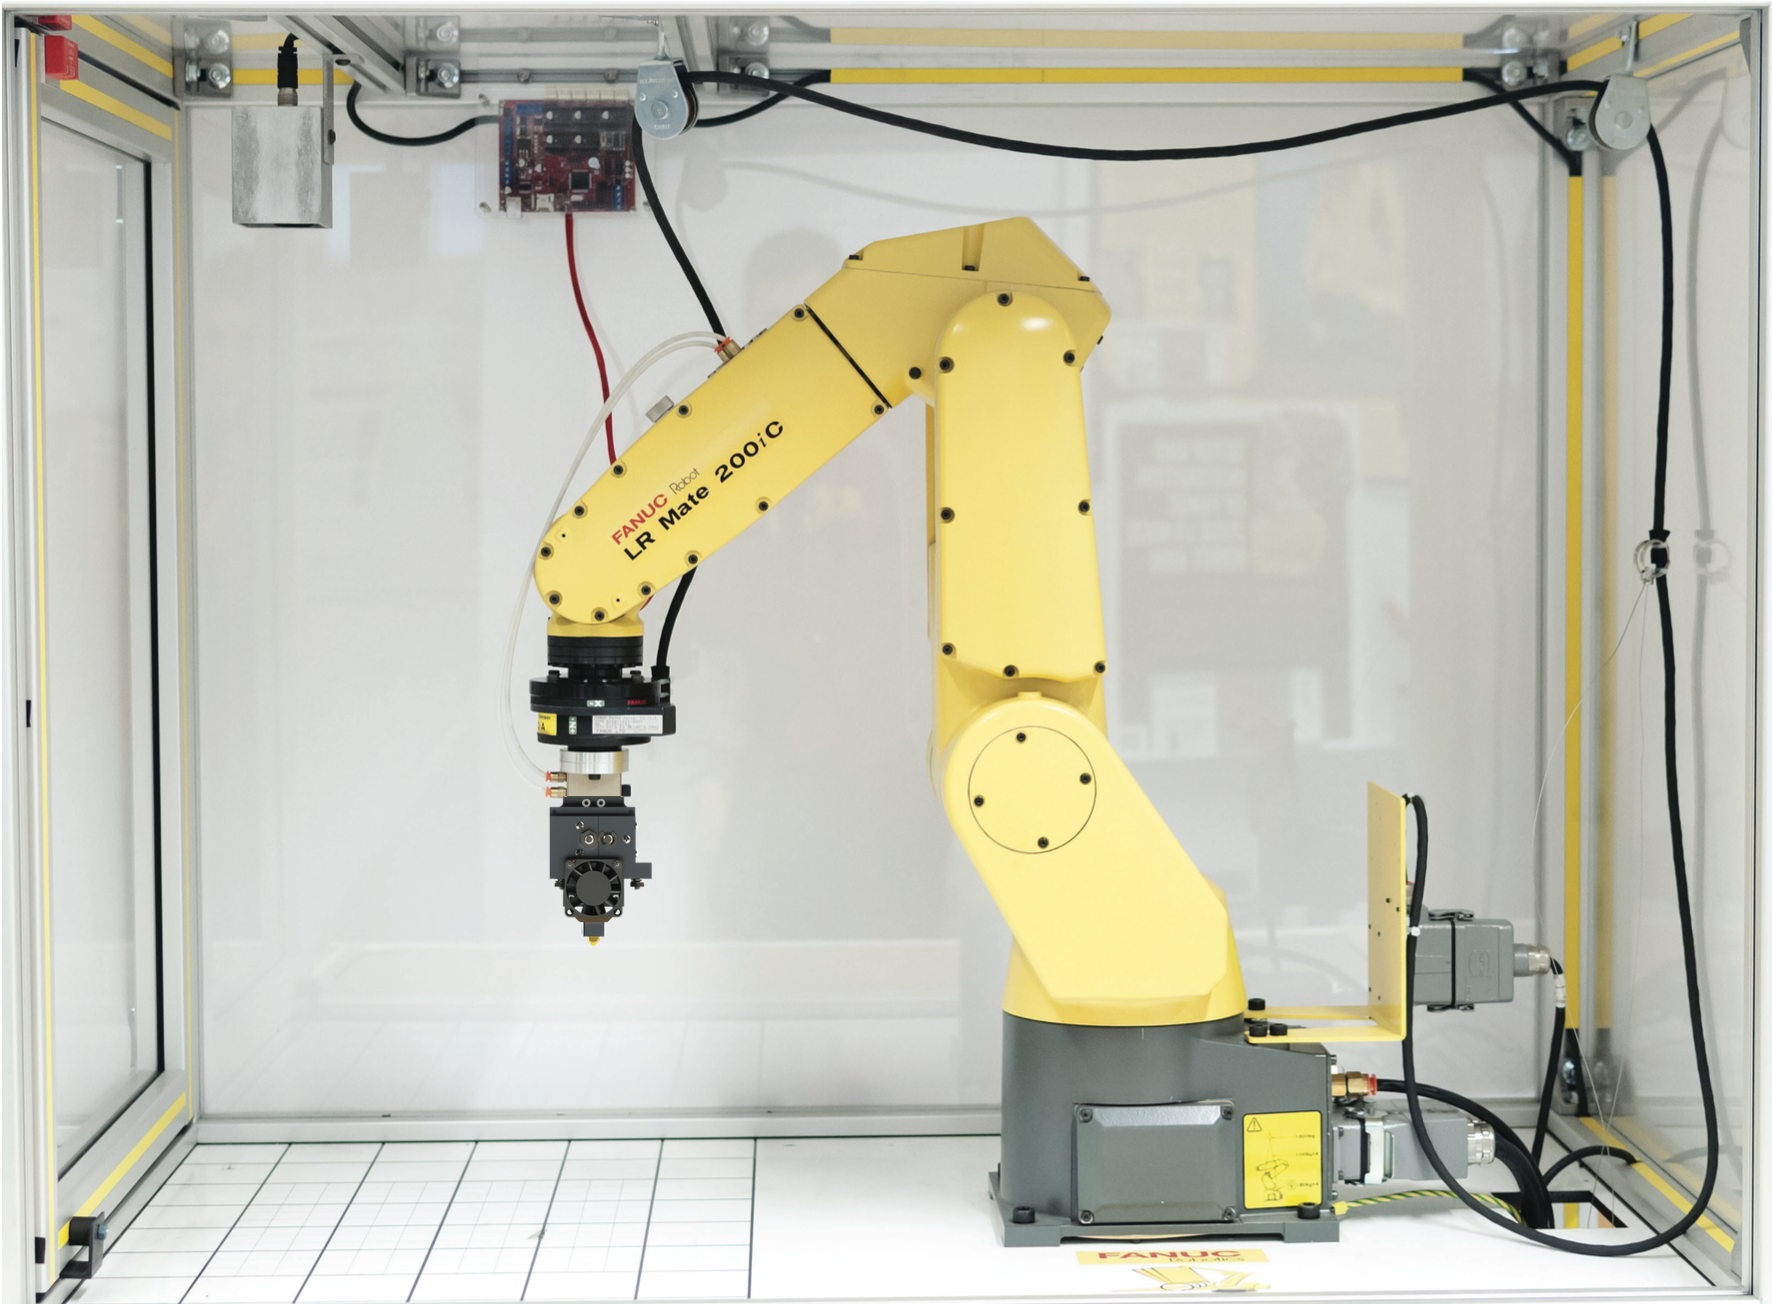
\includegraphics[width=0.5\textwidth]{./figures/robot-extruder-electronics}
\caption{A photograph of the robot with the mounted electronics and a rendering of the extruder.}
\label{fig:robot with things}
\end{figure}